\documentclass[a4paper]{article}

\usepackage[utf8]{inputenc}
\usepackage{fancyhdr}
\usepackage{geometry}
\usepackage[frenchb]{babel}
\usepackage{libertine}
\usepackage[pdftex]{graphicx}
\usepackage{hyperref}
\usepackage{slashbox}
\usepackage[T1]{fontenc}
\usepackage{multirow}
\usepackage{graphicx}
\usepackage{array,multirow,makecell}
\setcellgapes{1pt}
\makegapedcells
\newcolumntype{R}[1]{>{\raggedleft\arraybackslash }b{#1}}
\newcolumntype{L}[1]{>{\raggedright\arraybackslash }b{#1}}
\newcolumntype{C}[1]{>{\centering\arraybackslash }b{#1}}
\geometry{a4paper}
\geometry{top=3cm, bottom=3cm, left=3.5cm, right=3.5cm}

\begin{document}
\large
\begin{titlepage}
		\title{Cahier des charges Lucidity by The Chamallow}

		\author{ CLAUS Marion -  DELECROIX Thomas - GINANE Charles - MARCHAUD Laurent	} 

		
\end{titlepage}


\pagestyle{fancy}
\lhead{The Chamallow}
\rhead{Cahier des charges Lucidity}
\renewcommand{\footrulewidth}{0.4pt}
\lfoot{EPITA Supinfo}


 \begin{titlepage}
\centering
\maketitle

\includegraphics[scale=2.25]{engrenage.png}

  \end{titlepage}


\quad
\quad

\tableofcontents

\newpage

\section{Introduction}


    Voici le cahier des charges de notre premier projet. En effet, nous sommes tous les quatre en SUPinfo c’est-à-dire en première année de prépa. Nous avons donc, pour le deuxième semestre, un projet à réaliser et le sujet, pour ce projet, est libre.
Nous avons donc décidé à l’unanimité de développer un jeu vidéo .
Notre jeu sera un jeu de réflexion où le joueur devra interagir avec le décor pour trouver la solution et donc réussir à finir les différents niveaux.
Dans ce cahier des charges , vous trouverez la présentation de notre groupe composé de Thomas “Tetra” DELECROIX (chef de projet), Marion “Santa” CLAUS , Charles “GIGI” GINANE et Laurent “Aluxima” MARCHAUD.
Vous trouverez ensuite la présentation de notre projet, d’où vient-il ? Comment cette idée de jeu nous est-elle venue à l’esprit ? Ainsi que les domaines que nous développerons dans ce projet.
Nous avons, pour continuer, les logiciels que nous allons utiliser au cours de ce projet et les coûts de réalisation de ce projet.
Enfin il y aura le répartition des tâches et aussi l’avancement entre les différentes soutenances comme une sorte de feuille de route.
Ce projet est une étape essentielle à notre formation d’ingénieur car elle va mettre en valeur, d’une part le travail de groupe et la bonne entente et cohésion entre les différents membres du groupe, et d’autre part à découvrir de nouvelles connaissances en terme de langage informatique mais aussi d’approfondir nos connaissances déja acquises au cours de notre premier semestre.
Notre but final est en premier lieu, de développer un jeu mais aussi de ressortir de ce projet avec de nouvelles connaissances notamment en code, mais aussi sur des compétences de developpement 3D, et de connaître ce qu’est le travail en équipe .

\begin{flushleft}
Il ne nous reste plus qu’à vous souhaiter une bonne lecture !
\end{flushleft}


\quad
\begin {centering}

The Chamallow !

\end{centering}

\begin{centering}


\includegraphics[scale=0.25]{Logo.png}

\end{centering}
\newpage

\section{Présentation de "The Chamallow"}
	\subsection{Le groupe en lui-même }


    Notre groupe composé de Thomas “Tetra” DELECROIX, Charles “Gigi” GINANE, Marion “Santa” CLAUS et Laurent “Aluxima” MARCHAUD provient de la classe A2. Nous nous sommes mis ensemble dans l’optique de créer un groupe d’un niveau homogène.
Son nom provient du début des premières syllabes de nos prénoms: “Tho”, “Cha”, “Ma” et “Lau” transformé en “The Chamallow”.
 


	\subsection{Présentation personnelle de chacun}
		\subsubsection{Thomas "Tetra" DELECROIX }
			
L’an dernier j’étais en terminale S en spécialité informatique et sciences du numérique. J’ai déjà quelques connaissances sur certains langages de programmation, mis à part le CAML, Csharp et Python que nous avons traités pendant ce premier semestre à Epita, comme en HTML, JavaScript, CSS, ActionScript et un peu de domotique avec Arduino. Pour notre groupe ce projet va nous apprendre à travailler en groupe ainsi que communiquer entre nous. Personnellement ce projet va sûrement me permettre d'approfondir ma méthodologie, mon analyse, ma réflexion ainsi que mes connaissances dans des langages comme par exemple le Csharp. Etant chef de groupe je vais également avoir la responsabilité de la cohésion et la motivation du groupe ainsi que du respect des deadlines que nous nous fixons.



		\subsubsection{Marion "Santa" CLAUS}
			
Contrairement à une bonne majorité des étudiants d’EPITA, l’informatique m’intéresse depuis peu de temps. Cela a commencé en terminale quand ma curiosité m’a poussée en spécialité ISN. Ainsi, à mon arrivée à EPITA, j’avais fait un peu de programmation en Python et avais quelques connaissances en HTML. Donc quand j’ai appris que j’allais travailler en groupe pour coder un jeu vidéo, je me suis dit que c’était une opportunité à saisir, que je pourrais apprendre de nouvelles choses. Bien sûr le fait qu’il ait un temps limite fait de ce projet un challenge que je suis prête à relever. Si vous ne l'aviez pas compris, j’aime élargir mes connaissances, c’est pourquoi je m’occuperai essentiellement de la partie graphique, un domaine qui m’est totalement inconnu.

\newpage

		\subsubsection{Charles "Gigi" GINANE}
			

Moi c’est Charles sous le surnom GIGI , je viens de province (du Sud plus exactement) d’une terminale Scientifique spécialité Physique. Par curiosité je me suis intéressé petit à petit à l’informatique à l’âge de 12 ans dès que j’ai eu mon ordinateur personnel..
Par curiosité , j’ai découvert quelques langages informatiques tels que le C, le C++, le php, le html et le css que j’ai pu expérimenter lors des TPE en créant notre propre site internet.
J’ai étendu ma passion en donnant des cours au club informatique de Montélimar ou bien en m’occupant de retransmettre des match de boules lyonnaises sur internet en direct.
Le fait de travailler en groupe est un atout pour moi , je pourrai apprendre des choses que j’ignorais et aussi apporter des connaissances que les autres n’ont pas (notamment en LaTeX ! ).
L’idée de faire de faire un projet ne me fait pas peur et ce premier projet va m’apporter beaucoup de connaissances car l’entente avec les autres membres du groupe est parfaite.

		\subsubsection{Laurent "Aluxima" MARCHAUD}

Venant de terminale S spécialité informatique et sciences du numérique (ISN), j’ai déjà quelques bases en programmation C/C++, Python, Caml, php et html, acquises en cours ou par curiosité avant le lycée. L’idée de créer un jeu vidéo de A à Z est alors quelque chose qui me motive énormément, notamment dans l’apprentissage du Csharp, le respect de délais, l’organisation et le travail de groupe. Pour le moment, mon seul travail de groupe en informatique a été le projet d’ISN de l’année dernière, que j’ai fait en binôme avec un ami. Tout s’est extrêmement bien passé et nous avons presque décroché la note maximale ! J’espère alors que ce travail se déroulera aussi bien; pour cela il faudra s’impliquer au maximum et ne jamais baisser les bras.
Je m’attends donc à ce que, en un semestre, nous puissions développer un jeu fantastique, complet, et tout ça, bien évidemment, sans aucun bug !

\newpage

\section {Présentation du projet}
	\subsection{Origine}

En premier lieu, nous n’avions pas d’idée précise sur le jeu que nous allions faire, mais au cours du temps nous avons réussi à éliminer les choix qui ne nous convenaient pas. Nous avons alors retiré les jeux types RPG, RTS, MOBA. L’idée d’un jeu de réflexion/plateforme nous est venue. Nous pensions d’abord faire un jeu de création de mécanismes constitués d’objets du décor, avec l’idée de faire comme, dans le jeu Minecraft, des systèmes de redstone (liaisons de fils et de composants) mais nous y avons réfléchi et avons pensé qu’un tel jeu serait trop ambitieux et que nous n’aurions sûrement pas suffisamment de temps pour terminer ce projet. Nous nous sommes alors restreints à l’interaction avec le décor, tel que des boutons.


	\subsection{Nature}

    Notre ambition est donc de créer un jeu de réflexion/plateforme/puzzle. La vue du personnage serait à la première personne. L’environnement serait à première vue des sortes de salles closes dans lesquelles le joueur doit effectuer une suite d’actions en interaction avec le décor lui permettant de sortir de la salle et de passer à un niveau supérieur. Notre jeu s'inspirant du principe du jeu de réflexion “Portal”. La ressource primaire (épuisable) du jeu serait la “Lucidité” qui pourrait, par exemple, servir à avoir des interactions à distance avec les objets. Cette ressource serait récoltée en exploitant des sources, rares, présentes à certains endroits de la carte. La lucidité serait contenable en quantité limitée dans une bouteille spéciale que le joueur transportera dans son dos. Le jeu se rapprochant le plus du nôtre est Q.U.B.E. Ce dernier est basé sur la construction de plateformes grâce à des solides physiques comportant des propriétés particulières comme la déformation, l’assemblage, etc.
Cela se traduit par le déplacement d’objets, pression de boutons, déplacements, etc. Il faudra également penser à l’aspect multijoueur du jeu en créant un mode de jeu adapté. Les joueurs évolueront ensemble et devront impérativement s’aider et effectuer des actions ensemble pour finir chaque niveau.

\newpage
 
	\subsection{Buts et intérêts}

    Ce projet a pour but de nous initier premièrement au travail de groupe. De plus il nous permettra de découvrir de nouveaux logiciels comme Unity, Blender et d’approfondir nos connaissances en C\#, LaTeX, Php, HTML, et tous les langages que nous rencontrerons.
La programmation de ce jeu induira également l’usage de formules mathématiques et physiques pour l’application de mouvements des objets, des trajectoires, etc.

\quad
\quad


\begin{centering}

\includegraphics[scale=1]{Portal2.jpg}

\end{centering}

\quad
\quad

\begin{centering}

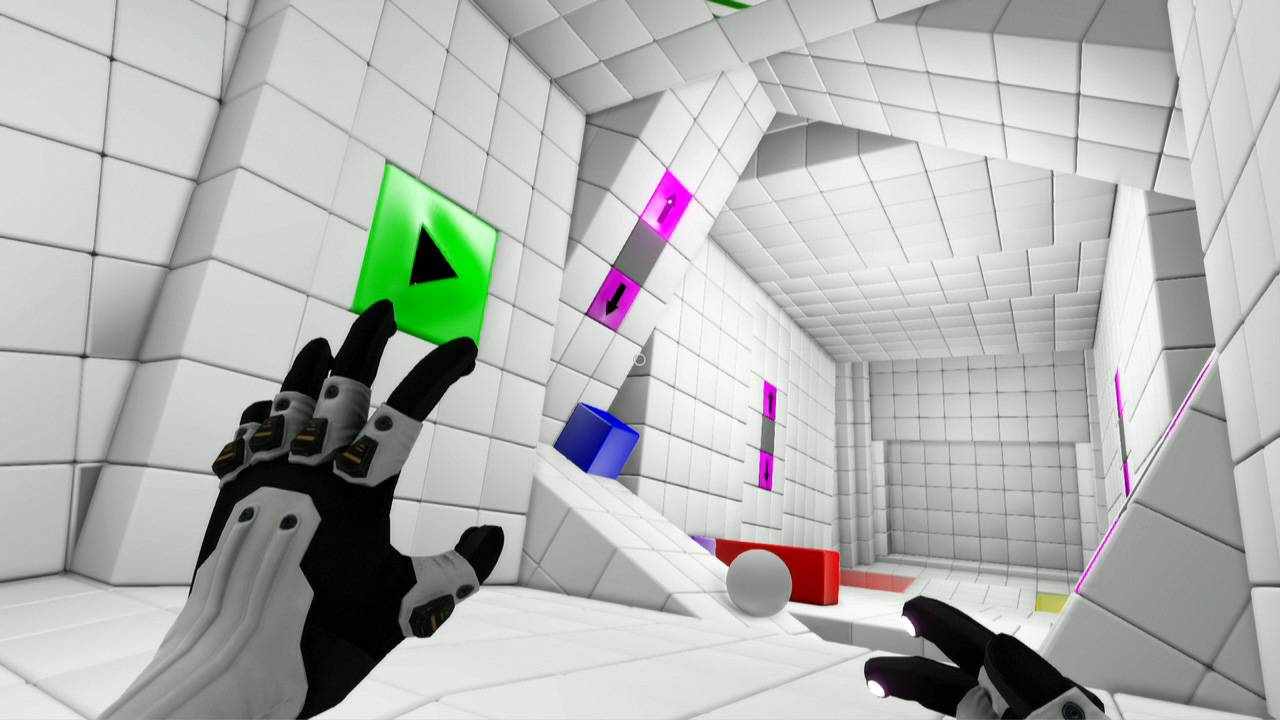
\includegraphics[scale=0.3]{qube.jpg}

\end{centering}

\newpage
\section{Description du projet}
	\subsection{Les points de notre projet}
Dans cette partie, nous allons vous présenter les differents points que nous utiliserons tout au long de notre projet. En voici la liste:

\quad

- \underline{Moteur Graphique :} Le moteur graphique inclus à Unity va nous permettre d’afficher les differentes structures visuelles présentes dans notre jeu.

\quad 

- \underline{Moteur Physique :} Ce moteur va permettre de gérer dans notre projet tout ce qui est collision entre le joueur et les murs, l’attraction de certains objets, la gravité dans le monde, le déplacement du personnage et des objets.

\quad

- \underline{Site :} Nous allons créer un site web sur lequel nous mettrons une présentation du projet et des membres du groupe, l’avancement du projet, comment nous contacter, des captures d’écran du jeu et les liens de nos sources. Il y aura aussi une version téléchargeable du jeu et un moyen pour s’inscrire/se connecter au jeu.

\quad

- \underline{Reseau :} Le reseau nous est nécessaire puisque nous avons l’ambition de faire un multijoueur ce qui nous oblige à adapter notre jeu.

\quad

- \underline{Gameplay :} Le gameplay est obligatoire dans tout jeu afin que le jeu soit jouable par une grande partie du public, c’est pour cela que nous le developperons et l’adapterons au cours de ce projet.

\quad

- \underline{Conception du monde :} Nous comptons créer differentes salles de difficultés différentes auquelles le ou les joueurs seront confrontés afin de parvenir à la fin du jeu.

\quad

- \underline{Son :} Le son est essentiel dans un jeu pour avoir une grande immersion. C’est pour cela que nous mettrons des musiques de fond pour l'ambiance, et des bruitages pour la réalité.

\quad

	\subsection{Résumé de nos objectifs}

Pour faire une conclusion sur cette partie qui nous paraît importante. Nous souhaiterons développer un jeu de type réflexion où l'on doit sortir d'une salle en s'aidant des différents décors. Nous développerons aussi un multijoueur
de type coopération où les deux joueurs devront s'entraider simultanément pour parvenir à la sortie et finir le ou les niveaux que nous leurs proposerons.
Le site internet proposera les dernières actualités de l'avancement de notre projet, le téléchargement de notre jeu disponible, quelques captures d'écrans de notre jeu, la présence de notre cahier des charges et enfin une petite présentation de notre jeu qui sera disponible.
\newpage

\section{Technologie}
	\subsection{Logiciels}
Les logiciels que nous comptons utiliser pour notre projet sont les suivants:

\quad
\quad

- \underline{Unity :} 
C’est le logiciel de base que nous utiliserons pour créer notre jeu. Ce logiciel permet de lier la 3D à du code. Le langage de programmation que nous allons utiliser est le Csharp, que nous avons appris récemment. C’est la première fois que nous allons utiliser ce logiciel. 

\quad

-\underline{Microsoft Visual Studio 2015 :}
C’est le logiciel que l’on utilise pour éditer notre code Csharp, nous avons déjà l’habitude de l’utiliser notamment en TP. 
Visual Studio est un bon logiciel vu qu'il est très simple à prendre en main notamment grâce aux erreurs qui sont détectées automatiquement et aux facilités du débugage.

\quad

-\underline{Blender:}
 Nous devrons avoir recours à Blender pour créer nos modèles 3D du jeu comme les personnages, les objets, le décor, etc.

\quad

-\underline{SourceTree :}
Travaillant en groupe, il va être indispensable d’organiser notre code afin de se répartir les tâches, repérer d’où viennent les éventuels problèmes, et créer des versions de notre jeu. Pour cela nous choisissons d’utiliser le système de Git qui nous permet de mettre en commun nos fichiers.

\quad

-\underline{Notepad++ :}
Il nous faudra évidemment un éditeur de texte simple et complet afin de mener à bien notre projet, Notepad++ devient alors indispensable !

\quad

-\underline{Skype :}
Un groupe skype a été créé dans le but de pouvoir garder contact même si nous sommes dans notre province originaire ou tout simplement en dehors d'EPITA, cela nous évite de communiquer par pigeon voyageur.
 
\quad

-\underline{Google Drive :}
Cet outil formidable nous permet d’écrire tous en même temps les documents que nous devrons rendre. Evidemment, cela ne nous sert que de support avant d’écrire le document en LaTeX.

\quad

-\underline{MiKTeX :}
C’est le logiciel que nous choisissons d’utiliser pour créer nos documents LaTeX.
LaTeX permet de générer un PDF simple et clair à l’aide de commandes faciles à utiliser.

\quad

-\underline{FileZilla :}
Il faudra nous connecter en FTP au serveur sur lequel le site web sera hébergé.

	\subsection{Coûts}

\begin{tabular}{|c|c|c|}
\hline Nom & Coût réel & Coût dépensé \\
\hline Microsoft Visual Studio 2015 & 13156€ & 0€ \\
\hline Unity & 0€ & 0€ \\
\hline MiKTeX & 0€ & 0€ \\
\hline Blender & 0€ & 0€\\
\hline SourceTree & 0€ & 0€ \\
\hline Adobe CC & 72€ & 0€\\
\hline Papier Encre & 80€ & 0€\\
\hline Nourriture & 3600€ & 3600€\\
\hline Total & 16908€ & 3600€\\
\hline
\end{tabular} 

\newpage

\section{Répartition des tâches / découpages}
	\subsection{Répartition des tâches}
\underline{Légende :} 


\quad
- = Pas de participation

 \quad
X = Faible implication

\quad
XX = Moyenne implication

\quad
XXX = Forte implication

 \quad

\begin{tabular}{|c||c|c|c|c|}
\hline Domaine / Nom & Laurent & Charles & Marion & Thomas \\ 
\hline Moteur graphique & - & - & XXX & X\\
\hline Moteur physique & - & - & - & XX\\
\hline Site & XXX & X & - & -\\
\hline Réseau & X & - & - & XXX\\
\hline Gameplay & - & XXX & X & -\\
\hline Conception du monde & XX & - & XX & -\\
\hline Son & - & XX & - & -\\
\hline


\end{tabular}

	\subsection{Avancement du projet par soutenances}

\underline{Légende :} 

\quad
- = Non debuté

 \quad
+ = commencé 

\quad
++ = Avancement important 

\quad
+++ = Domaine fini

 \quad

			\begin{tabular}{|c|c|c|c|}
\hline Domaine & 1ère Soutenance & 2ème soutenance & 3ème soutenance \\
\hline Moteur graphique & ++ & ++ & +++\\
\hline Moteur physique & ++ & +++ & +++\\
\hline Site & ++ & +++ & +++\\
\hline Réseau & - & ++ & +++\\
\hline Gameplay & + & ++ & +++\\
\hline Conception du monde & + & ++ & +++\\
\hline Son & + & ++ & +++\\
\hline Finalisation & - & ++ & +++ \\
\hline
			\end {tabular}

\newpage
\section{Conclusion}


Ce projet va nous mener à apprendre par nous-même ainsi que faire les recherches nécéssaires donc nous allons mieux retenir tout ce que nous verrons pour résoudre nos problèmes.
Maintenant que nous somme fixés sur nos objectifs à atteindre pour Lucidity. 
Nous comptons énormement sur ce projet pour améliorer nos connaissances en langage informatique et en découvrir de nouvelles.
Ce projet nous donnera aussi une première expérience sur ce qu'est le travail de groupe en informatique.
La théorie est maintenant fini, place maintenant à la pratique, il ne nous reste plus qu’à plonger dans ces lignes de code.

\quad

\centering
\LARGE 

THE CHAMALLOW



\end{document}